\section{Kinematika}
\paragraph{Enakomerno pospešeno gibanje} (\(\ds a := \frac{dv}{dt} = \text{const}\)).
%
\begin{itemize}
    \item \(\ds dv = a \, dt \lthen \int_{v_0}^{v} \, dv = a \int_{0}^{t} \, dt \lthen v - v_0 = at \lthen  \boxed{v = v_0 + at}\)
    \item \(\ds v := \frac{ds}{dt} \lthen ds = (v_0 + at) \, dt \lthen \int_{0}^{s} \, ds = \int_{0}^{t} (v_0 + at) \, dt \lthen \boxed{s = v_0t + \frac{1}{2}at^2}\)
    \item \(\ds v = \frac{ds}{dt}, \ a = \frac{dv}{dt} \lthen v \, dt = ds, \ a \, dt = dv \lthen \frac{v}{a} = \frac{ds}{dv} \lthen v \, dv = a \, ds \lthen \int_{v_0}^{v} v \, dv = \int_{0}^{s} a \, ds\)
    
    \(\ds \lthen \frac{v^2}{2} - \frac{v_0^2}{2} = as \lthen \boxed{v^2 - v_0^2 = 2as}\) (če imamo delo z pojemkom, spremenimo predznak)
    \item \textbf{Enakomerno gibanje:} Vzemimo \(a = 0\)
\end{itemize}
%
\paragraph{Prosti pad} (\(v_0 = 0, \  g = 9.8 \  \text{m} / \text{s}^2\)).
\begin{itemize}
    \item \(\ds \boxed{v = gt, \ t = \sqrt{\frac{2h}{g}}, \ h = \frac{1}{2} g t^2}\)
\end{itemize}

\paragraph{Relativna hitrost:} \(\vec{v}_r = \vec{v}_1 - \vec{v}_2, \ v_r = |\vec{v}_1 - \vec{v}_2|\)
%

\paragraph{Vodoravni met}
\ 

\begin{minipage}[t]{0.35\textwidth}
    \vspace{0pt}
  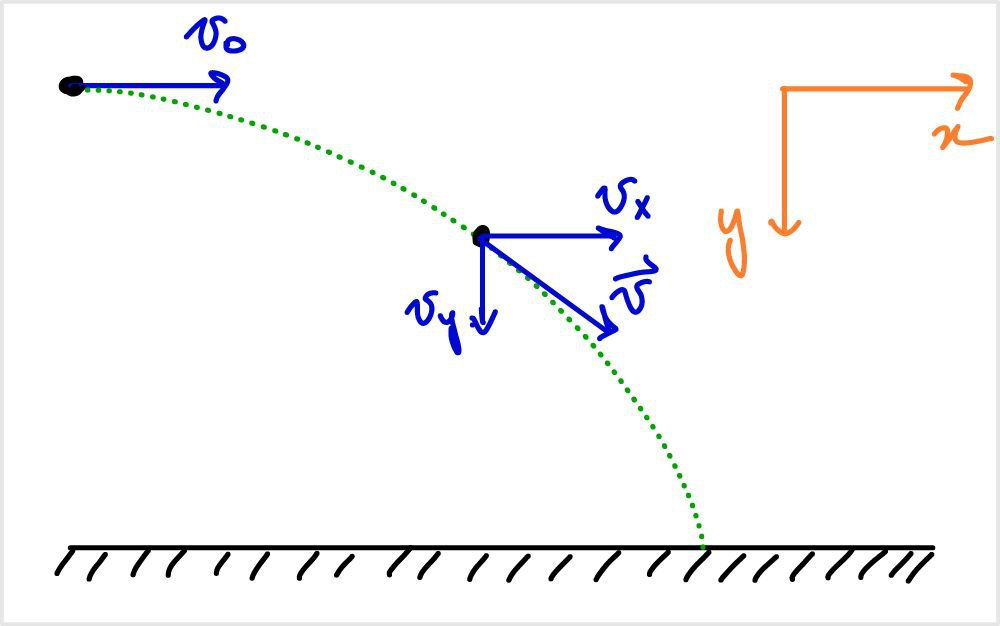
\includegraphics[width=\linewidth]{img/01_001.jpg} 
\end{minipage}
\hfill
\begin{minipage}[t]{0.60\textwidth}
    \vspace{0pt}
    \begin{itemize}
        \item \(x(t) = v_0 t, \ y(t) = \frac{1}{2}gt^2\)
        \item \(v_x = v_0 = \text{const}, \ v_y(t) = gt\)
    \end{itemize}
\end{minipage}
%
\paragraph{Poševni met}
\ 

\begin{minipage}[t]{0.35\textwidth}
    \vspace{0pt}
  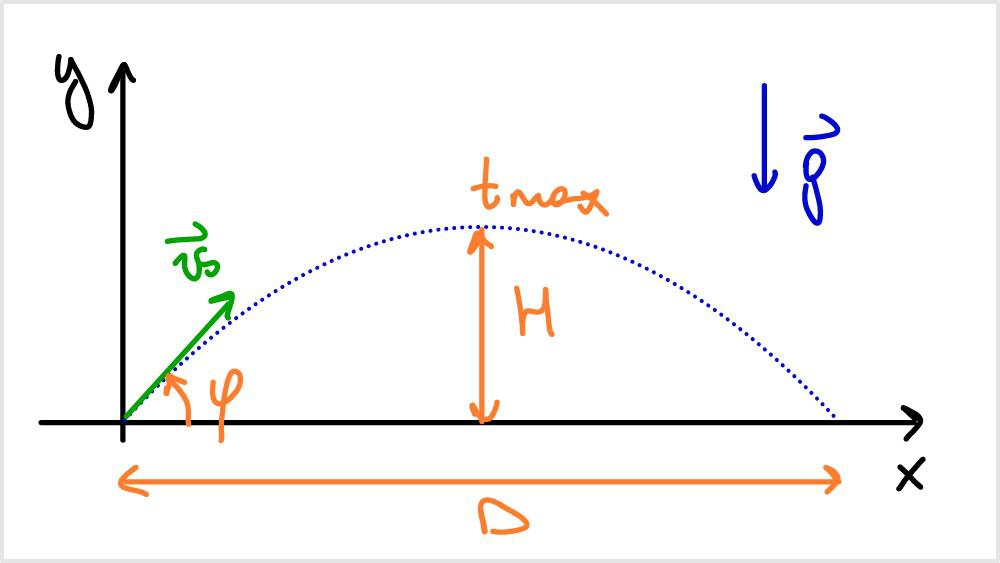
\includegraphics[width=\linewidth]{img/01_002.jpg} 
\end{minipage}
\hfill
\begin{minipage}[t]{0.60\textwidth}
    \vspace{0pt}
    \begin{itemize}
        \item \(x(t) = v_0 t \cos \phi, \ y(t) = v_0 t \sin \phi - \frac{1}{2}gt^2\)
        \item \(v_x = v_0 \cos \phi, \ v_y(t) = v_0 \sin \phi - gt\)
        \item \(\boxed{t_\text{max} = \frac{v_0 \sin \phi}{g}, \ D = \frac{v_0^2 \sin 2 \phi}{g}, \ H = \frac{v_0^2\sin^2 \phi}{2g}}\)
        \item Gibanje lahko razdelimo na dva dela: do \(H_\text{max}\) (poševni met) in po \(H_\text{max}\) (vodoravni met)
        \item Vodoravni met je posebni primer poševnega meta pri \(\phi = 0\)
    \end{itemize}
\end{minipage}
%
\paragraph{Kroženje}
\ 

\begin{minipage}[t]{0.25\textwidth}
    \vspace{0pt}
  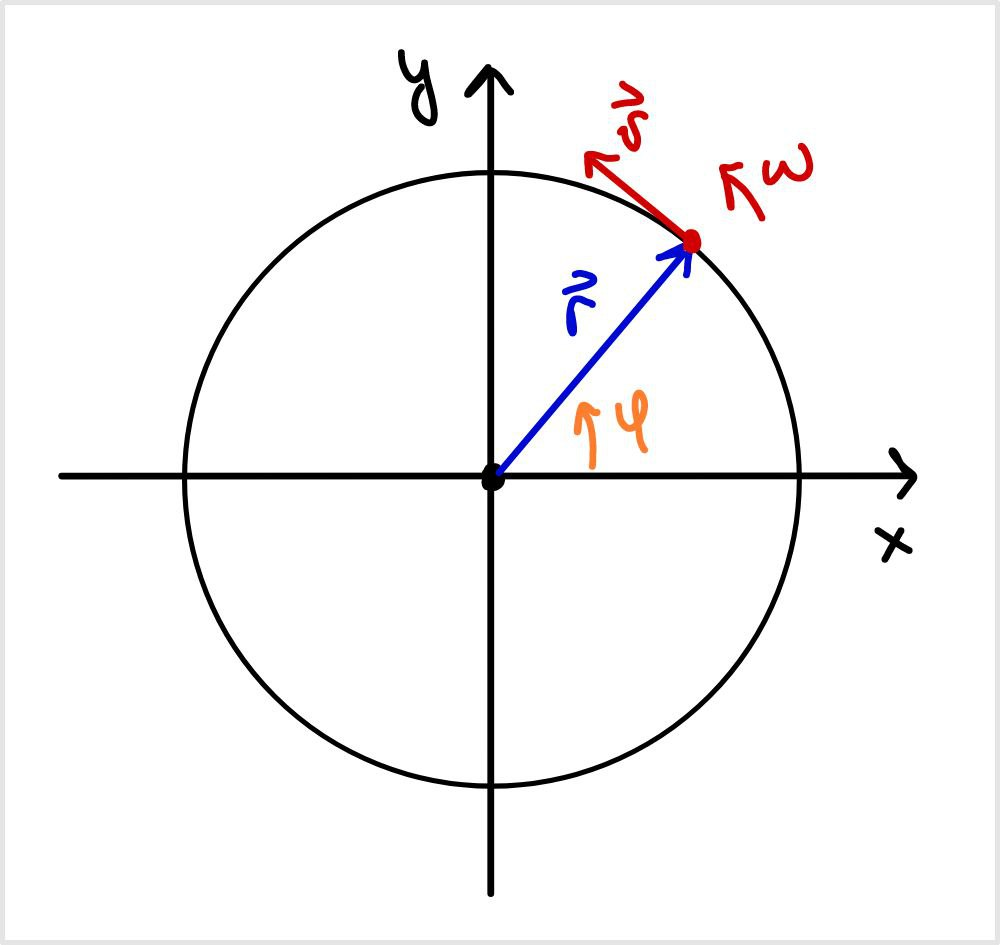
\includegraphics[width=\linewidth]{img/01_003.jpg} 
\end{minipage}
\hfill
\begin{minipage}[t]{0.70\textwidth}
    \vspace{0pt}
    \begin{itemize}
        \item \(\vec{r}(t) = r (\cos \phi, \sin \phi), \ \vec{v}(t) = r \omega (-\sin \phi, \cos \phi)\), kjer \(\omega = \dot{\phi}\) \emph{kotna hitrost}
        \begin{itemize}
            \item \(s = r \phi\), če merimo \(\phi\) v radianih
        \end{itemize}
        \item \(a(t) = r \alpha (-\sin \phi, \cos \phi) + r \omega^2 (-\cos \phi, -\sin \phi)\), kjer \(\alpha = \ddot{\phi}\) \emph{kotni pospešek}
        \begin{itemize}
            \item \(\vec{a}_t = r \alpha (-\sin \phi, \cos \phi)\) je tangentni pospešek (spreminjanje velikosti \(\vec{v}\))    
            \item \(\vec{a}_r = r \omega^2 (-\cos \phi, -\sin \phi)\) je radialni pospešek (spreminjanje smeri \(\vec{v}\))        
        \end{itemize}
        \item \(\ds \boxed{v = r \omega,\ a_t = r \alpha, \ a_r = r \omega^2 = \frac{v^2}{r}, \ a = \sqrt{a_r^2 + a_t^2}}\)
        \item \(\ds \omega = 2 \pi \nu, \ \nu = \frac{1}{t_0}\), kjer \(t_0\) je čas enega obrata, \(\nu\) je \emph{frekvenca}
        \item Enakomerno pospešeno kroženje ima iste enačbe kot enakomerno pospešeno gibanje
    \end{itemize}
\end{minipage}

\paragraph{Vektorski opis kroženja}
\begin{itemize}
    \item Definiramo \(\vec{\phi} = (0, 0, \phi)\) (smer \(\vec{\phi}\) lahko dobimo po pravilu desnega vijaka), potem
    \begin{itemize}
        \item \(\vec{v} = \vec{\omega} \times \vec{r}\)
        \item \(\vec{a} = \vec{\alpha} \times \vec{r} + \vec{\omega} \times (\vec{\omega} \times \vec{r})\)
    \end{itemize}
\end{itemize}

\paragraph{Splošno gibanje}
\begin{itemize}
    \item \(\ds R = \frac{v^2}{a_r}, \ \omega = \frac{a_r}{v}, \ \alpha = \frac{a_t a_r}{v^2}\) (vsako gibanje je trenutno kroženje), \(a_t, a_r\) sta komponenti \(g\)
\end{itemize}

\paragraph{Splošni nasveti}
\begin{itemize}
    \item Lahko obrnemo čas (začetek = konec)!
\end{itemize}